Dieser Teil wird beschreiben, wie der Schuldrucker zusammen gebaut wurde, was justiert werden musste, wie die Elektronik angeschlossen ist etc.
Er kann somit teilweise auch zum Troubleshooting verwendet werden, dient allerdings hauptsächlich der Dokumentation.

Der Drucker, mit dem sich dieses Handbuch befasst, ist ein "`GeeTech Prusa i3"'. Dies ist ein "`No-Name"' DIY-Kit zum Zusammenbau eines 3D-Druckers, und kann sich daher jederzeit vom Materialinhalt ändern. Sollte man dementsprechend auf Basis dieses Handbuches seinen eigenen Drucker zusammen bauen wollen, so muss man damit rechnen dass einige Dinge nicht exakt diesen Beschreibungen entsprechen. Es ist immer besser, im Internet nach der aktuellsten Bauanleitung zu suchen, doch selbst diese können eventuell nicht aktuell sein. 3D-Drucker-Zusammenbau ist meist verbunden mit Improvisation und Intuition.

Dies gesagt kann die verwendete, ausführlichere Bauanleitung des Herstellers hier gefunden werden:\\
https://goo.gl/DmXHE7
\begin{center}

\includegraphics{Bilder/Anleitung_QRCode.png}
\end{center}
Im folgenden werden durchaus einige der Bilder des Tutorials für bessere Verständlichkeit genutzt. Diese sind deutlich an den schwarzen Teilen des Druckers erkennbar. Der schulische Drucker hat durchsichtige Acrylglas-Platten, und kann so unterschieden werden.


\subsubsection{Schritt 0: Das Material}
Nach öffnen der Boxen standen uns folgende Materialien zur Verfügung:
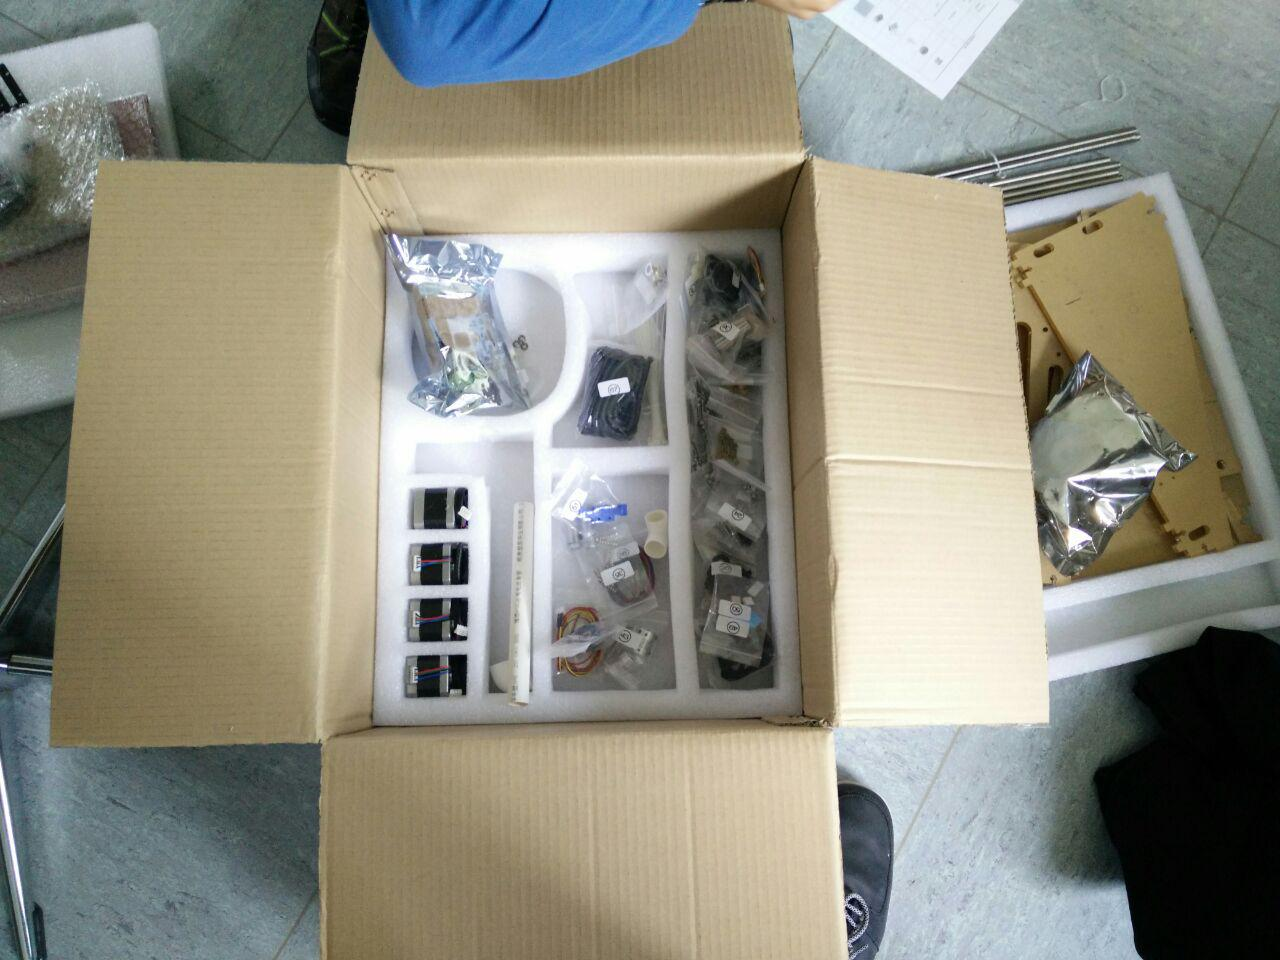
\includegraphics[clip=true,trim=230 100 320 100,angle=90,width=\textwidth]{Bilder/Material_1.jpg}
Enthalten hierin waren:
\begin{itemize}[noitemsep]
\item 4x NEMA17 Schrittmotoren
\item Die Kupplungen (Verbindungelemente zwischen Schrittmotor und Z-Achse)
\item GT2 Pulleys
\item X-Achen-Pulley-Verbinder (blaues Plastikteil)
\item Das GeeeTech GT2560 Steuerboard
\item Kabelbinder und Spiralschlauch
\item Lüfter und passende Kabel
\item Verschiedene Schrauben (M3)
\item Linearlager (8mm Innendurchmesser)
\item Teile für die Filamentrollenhalterung (Plastikrohre)
\end{itemize}
\vspace{\linewidth}
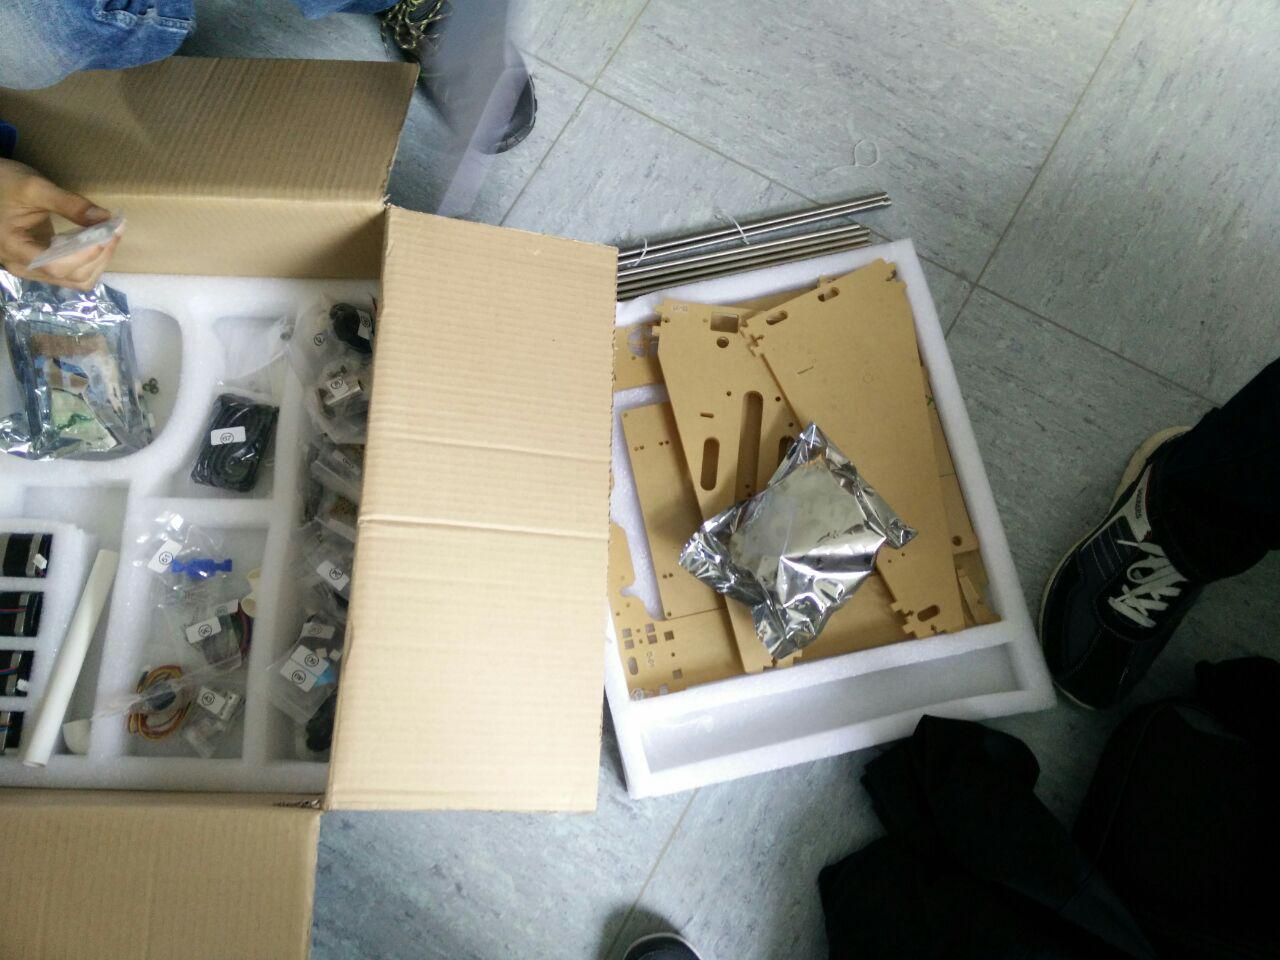
\includegraphics[clip=true,trim=410 100 150 100,angle=90,width=\textwidth]{Bilder/Material_2.jpg}
In dieser Packung enthalten waren:
\begin{itemize}[noitemsep]
\item Die verschiedenen Acryl-Platten
\subitem 4x Y-Achsen-Platten
\subitem XZ-Achsen-Frame
\subitem 2x XZ-Y-Verbinder-Platten
\subitem Heizbett-Platte
\subitem 2x Z-Achsen-Motor-Befestigungen
\subitem Die Platten des Filamentrollen-Halters
\subitem Sowie das LC-Display-Befestigungsmaterial

\item Die verschiedenen Linear-Stangen
\subitem Glatte Stahlstangen verschiedener Länge
\subitem 2x M8-Gewindestangen für die Z-Bewegung
\subitem 2x M8-Gewindestangen für den Y-Achsen-Aufbau
\end{itemize}
\vspace{\linewidth}
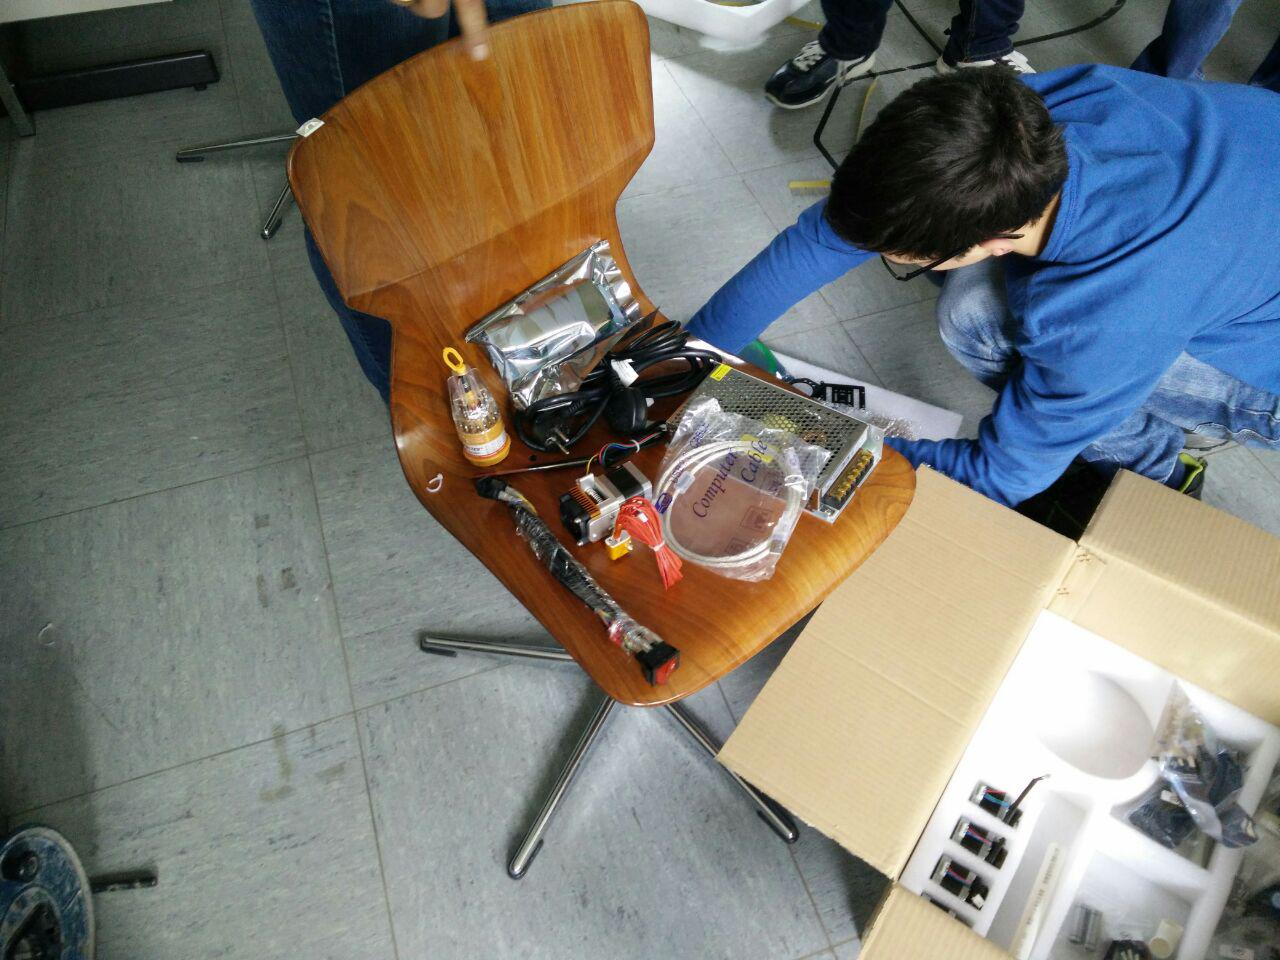
\includegraphics[clip=true,trim=260 180 230 160,width=\textwidth]{Bilder/Material_3.jpg}
Hier zu finden sind:
\begin{itemize}[noitemsep]
\item Das Netzteil, inklusive Stromkabel und Verbindungskabel mit Schalter
\item Den Extruder-Aufbau (mitsamt Motor, Hotend, Düse etc.)
\item Das Drucker LC-Display, über welches sich dieser steuern lässt, bzw. mit dessen Hilfe über SD-Karte gedruckt werden kann.
\item Das beiliegende Schraubendreher-Set
\item Das USB-Kabel zur Verbindung des GT2560 mit einem geeigneten Computer bzw. Pi
\item Einige Metallteile, z.B. die X-Schlitten-Platte
\end{itemize}

\newpage
\subsubsection{Schritt 1: Aufbau der Y-Achse}
Der obig verlinkten Anleitung folgend wurde beim Aufbau des Druckers zuerst die Y-Achse zusammen gebaut.
Hierfür wurden anfangs die nötigen Schrauben und Verbinder-Teile auf die zwei M8-Gewindestangen geschraubt:
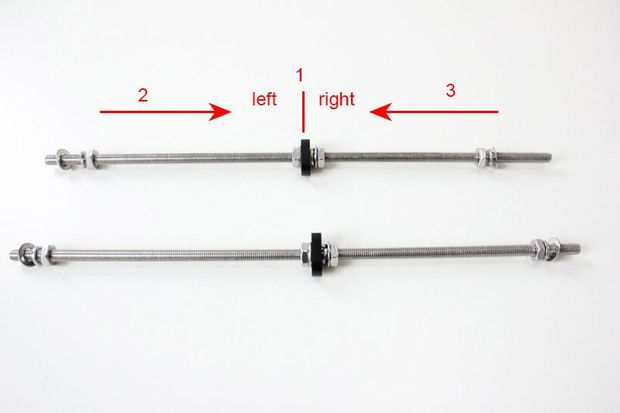
\includegraphics[clip=true,trim=0 100 0 40,width=\textwidth]{Bilder/Y_Assembly_Tutorial_1.jpg}

Als nächstes wurden die zwei Linear-Stangen zusammen mit den Y-Endplatten festgeschraubt. Wichtig ist, dass die Linearlager schon vorher auf die Stangen gesteckt werden!\\
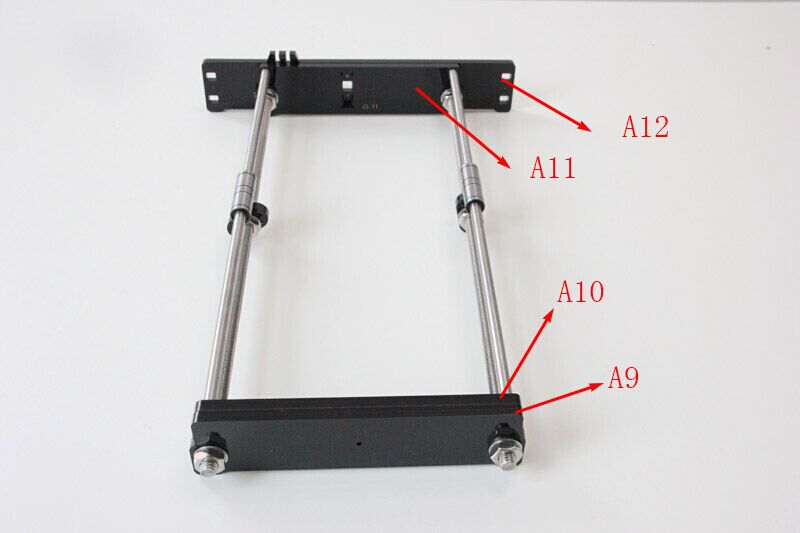
\includegraphics[width=\textwidth]{Bilder/Y_Assembly_Tutorial_2.jpg}

Anschließend wurde der Y-Schrittmotor, sowie die Riemenführung, an das nun fertige Y-Frame angebracht:\\
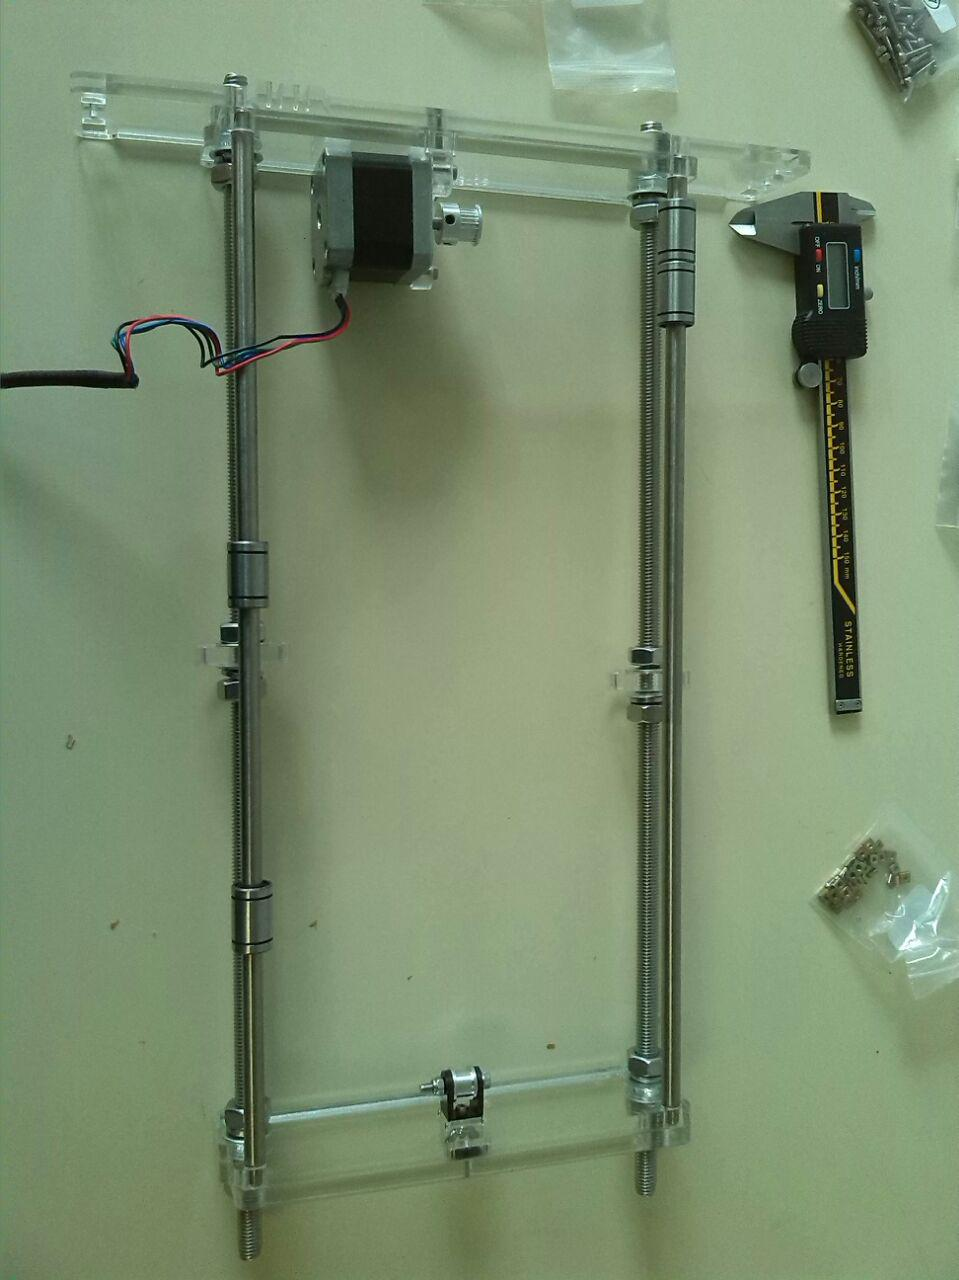
\includegraphics[clip=true, trim=30 0 100 0, angle=90, width=\textwidth]{Bilder/Y_Assembly_1.jpg}

Zum Abschluss wurde nun die Heizbett-Halterung mithilfe von Kabelbindern auf die Linearlager der Y-Achse angebracht, und der GT2-Treibriemen mit Bett-Halterung und Motor verbunden.\\
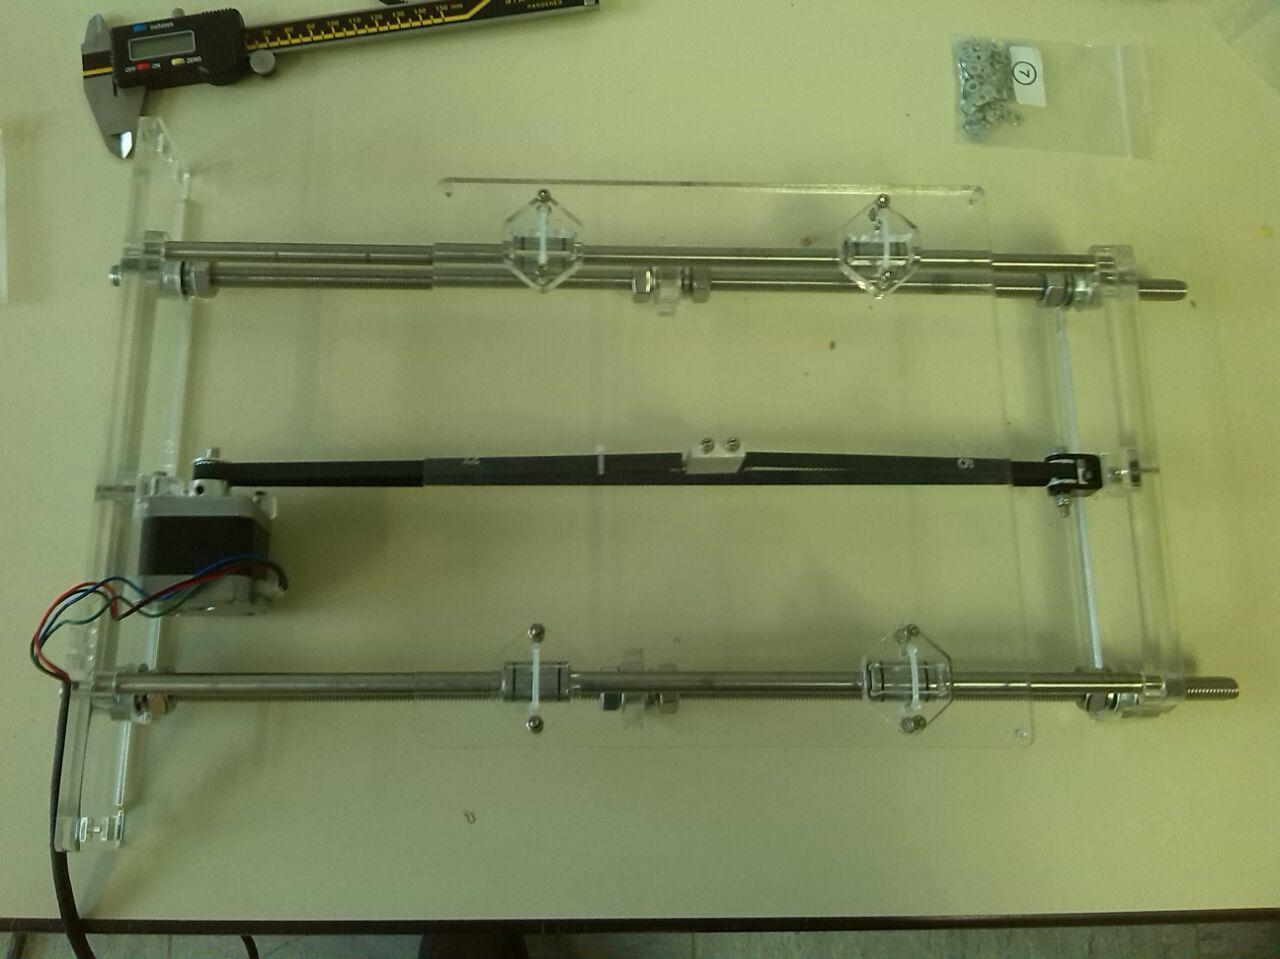
\includegraphics[clip=true, trim=0 40 0 40, angle = 0, width=\textwidth]{Bilder/Y_Assembly_Bed.jpg}

\subsubsection{Schritt 2: Aufbau der Y-Z-Einheit}
Nachdem die Basis des Gestells, die Y-Achse, fertig gebaut war, konnte angefangen werden die Z-Achse auf zu bauen. Hierzu wurde die Hauptplatte an die vorher auf die Y-Achse geschraubten Verbinder-Teile angeschraubt. Wichtig war hierbei ein korrekter Abstand zu der hinteren Y-Achsen-Platte, um einen geraden Aufbau des Druckers zu gewährleisten. Dies konnte mithilfe einiger weiterer Acryl-Teile erreicht werden, welche danach angebracht wurden.\\
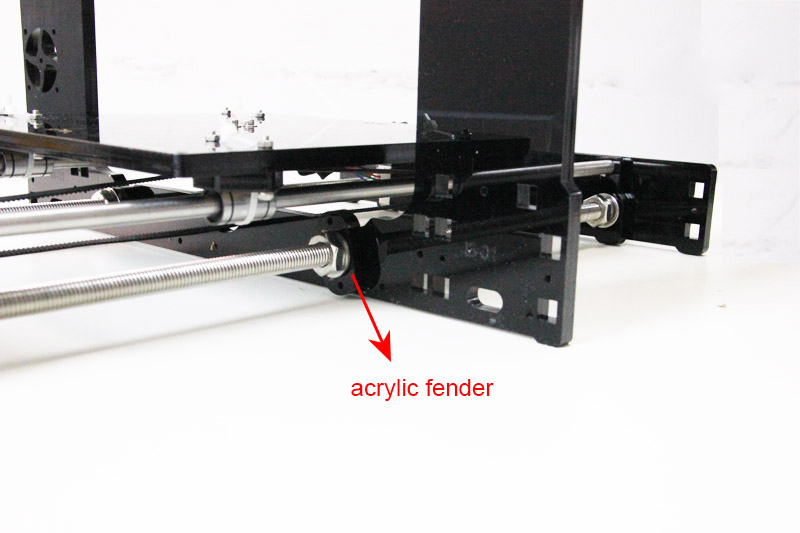
\includegraphics[clip=true, trim= 0 0 0 0, angle=0, width=\textwidth]{Bilder/Z_Assembly_1.jpg}

Nun wurden die vorher erwähnten Teile, zwei verbindende Seiten-Platten, zwischen die Hauptplatte und der hinteren Y-Achsen-Platte geschraubt. Wichtig war, dass auf die Ausrichtung geachtet wurde, um die Platte für die Stromversorgung auf die rechte Seite des Druckers zu bringen:\\
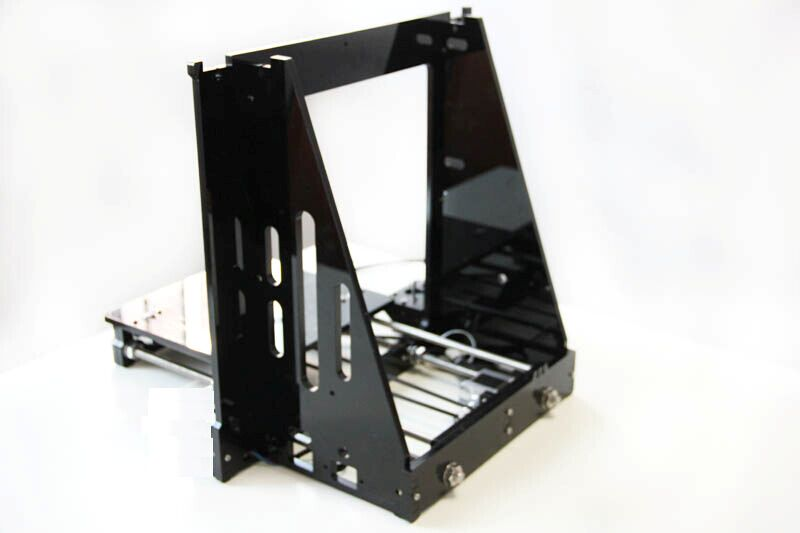
\includegraphics[width=\textwidth]{Bilder/Z_Assembly_2.jpg}
Die Verbindungen zwischen beiden Platten wurde mithilfe von M3-Schrauben und Muttern erledigt.

\subsubsection{Schritt 3: Aufbau der Z-Motoren}
Mit der Hauptplatte fest und gerade angebracht konnte nun die Z-Achse befestigt werden. Dies beinhaltet den Aufbau der Motor-Halterungen, sowie die zwei Linearachsen und die Gewindestangen, mit welchen der Druckkopf angehoben oder gesenkt werden kann.

Zuerst wurden hierfür mithilfe einiger Acryl-Teile die Motorhalterungen an die Hauptplatte angebracht.
Wichtig war hierbei zu beachten, dass eine Seite eine Halterung für einen Z-Endstop hatte, die andere jedoch nicht!\\
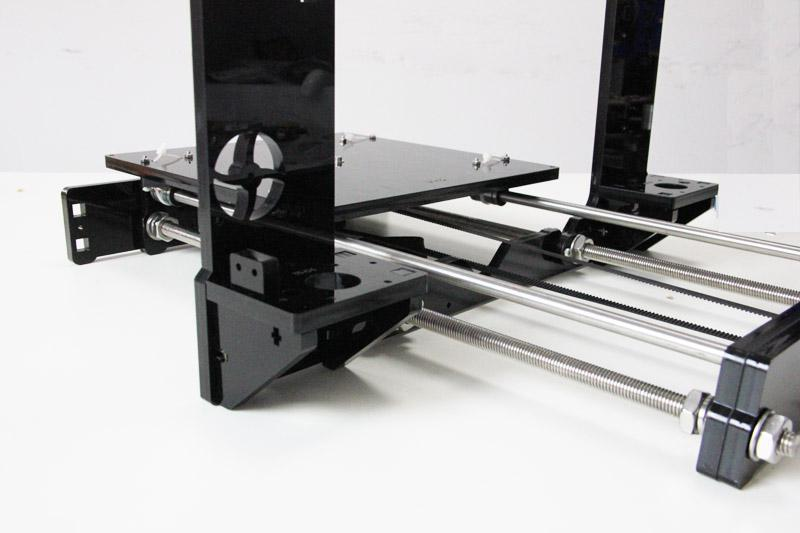
\includegraphics[clip=true, trim=30 100 0 0, width=\textwidth]{Bilder/Z_Assembly_3.jpg}

In diese Halterungen wurden nun die Motoren eingebaut. Wichtig war, dass die Motor-Kabel durch die dafür vorgesehenen Führungslöcher geleitet wurden!\\
\begin{center}
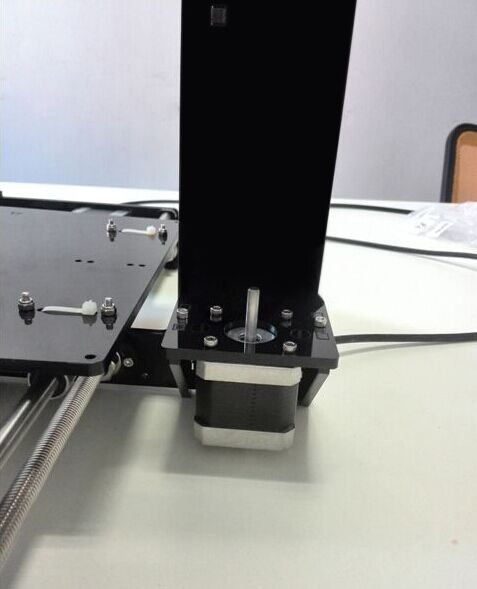
\includegraphics[clip=true, trim=30 60 30 130, width=0.7\textwidth]{Bilder/Z_Assembly_4.jpg}
\end{center}

\subsubsection{Schritt 4: Aufbau der X-Achse}
Bevor die Z-Achse fertig gestellt werden kann, muss zuerst die X-Achse aufgebaut werden, da diese später auf die Z-Achsen geschoben werden muss, bevor diese zusammen geschraubt wird!! 
Wichtig ist auch zu bemerken: Im Online-Tutorial wurden für die X-Achsen-Teile 3D-Gedruckte Teile verwendet. Der Schul-Drucker hat jene Teile nicht, stattdessen wurde er komplett aus Aluminium-Teilen gefertigt!

Die X-Achse wurde dazu wie folgt aufgebaut:
Die zwei Linearlager wurden auf die Linearstangen geschoben, zusammen mit zwei Befestigungsmuttern. Hiernach wurden die zwei X-Achsen-Befestigungen auf die Seiten der Stangen aufgeschoben. An ihnen beiden wurden jeweils ein Linearlager und eine spezielle Gewindemutter mit Befestigungsflansch angebracht, zusätzlich wurde an dem linken Endstück die Riemenführrolle befestigt.
Das Endergebnis sollte dementsprechend so aussehen:\\
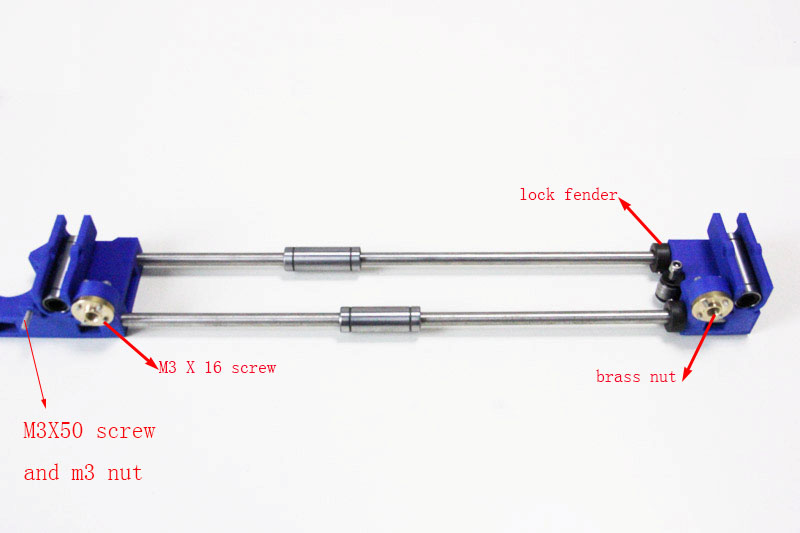
\includegraphics[clip=true, trim=0 0 0 100, width=\textwidth]{Bilder/X_Assembly_1.jpg}

\paragraph{Anmerkung:} Im Folgenden unterscheiden sich Online-Anleitung und der schulische Drucker stark. Z.B. erfordert die Online-Anleitung ein Zusammenbau des Extruders. Dies war für den Schul-Drucker nicht nötig. Dennoch sind viele der Schritte sehr ähnlich.

Zuerst wurde der X-Schlitten mithilfe von Kabelbindern auf die X-Achse angebracht:\\
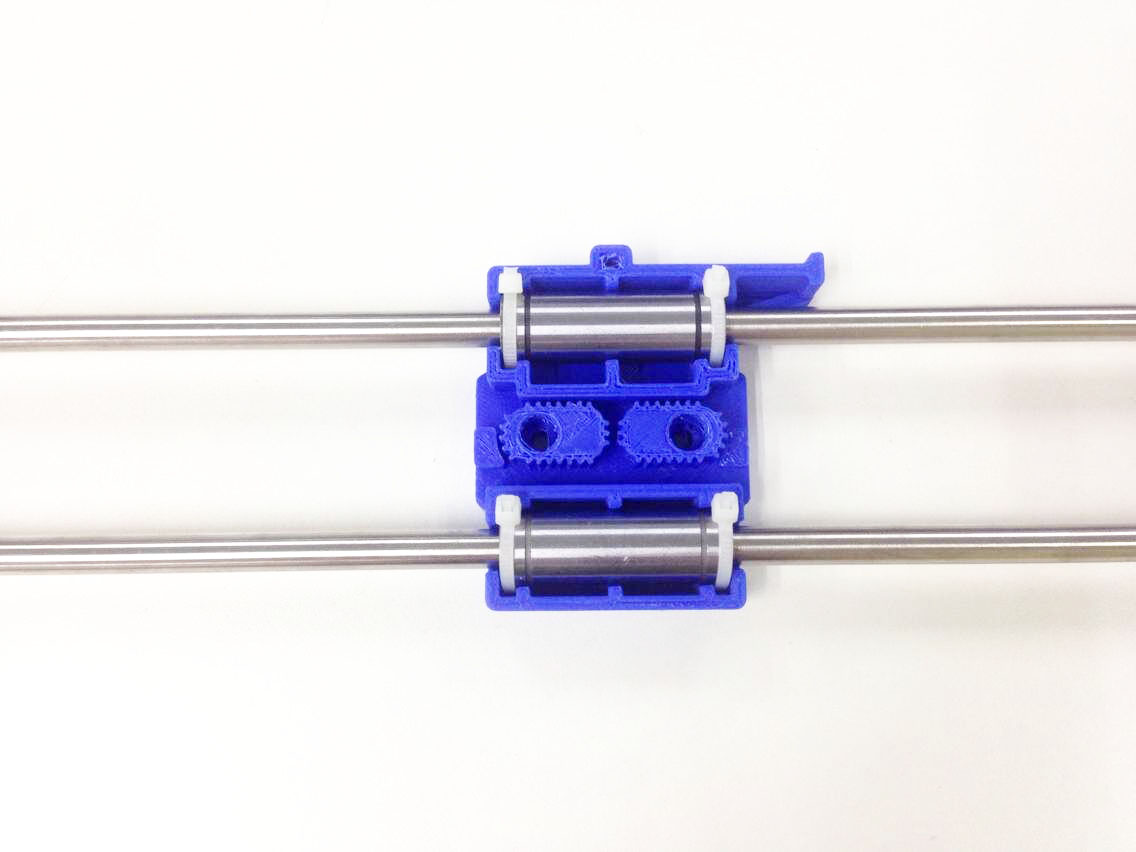
\includegraphics[clip=true, trim= 0 0 0 0, width=\textwidth]{Bilder/X_Assembly_2.jpg}
Da nun der Extruder bereits komplett zusammen gesetzt worden war, konnte dieser direkt auf dem X-Achsen-Schlitten angebracht werden.

Der nächste Schritt war nun das anbringen des Motors und des Treibriemens.\\
\begin{tabular}{ccc}
 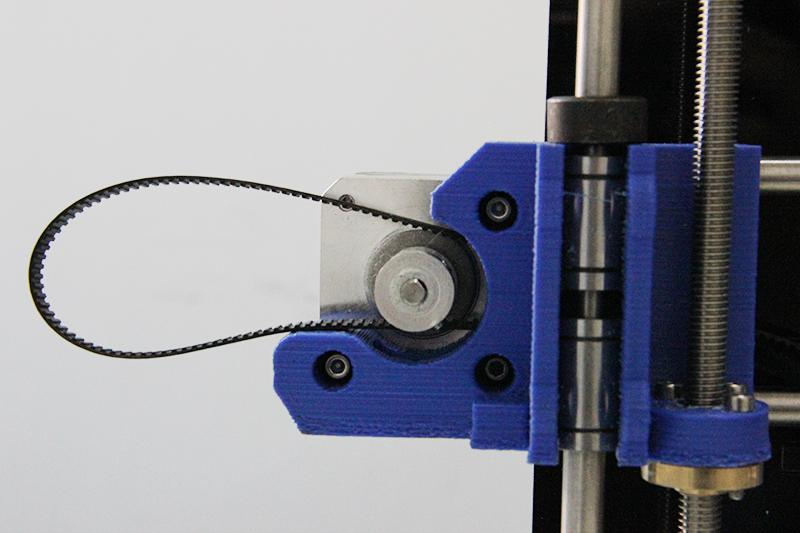
\includegraphics[width=0.3\textwidth]{Bilder/X_Belt_1.jpg} & 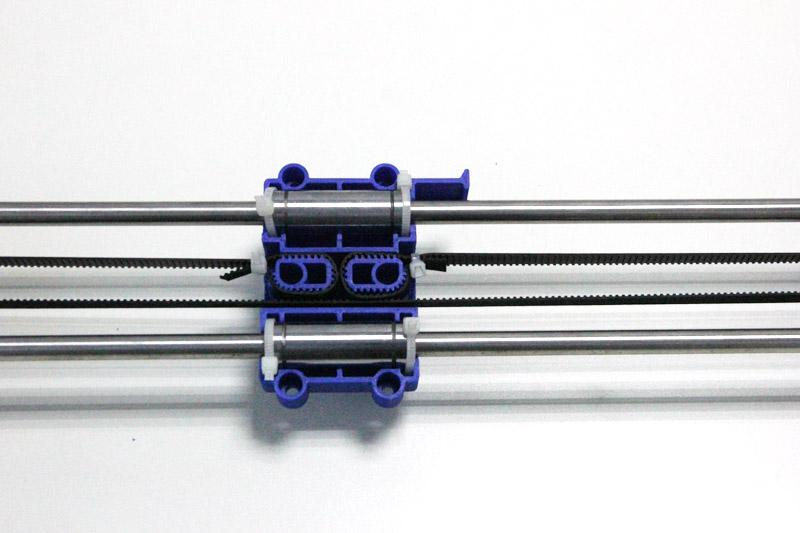
\includegraphics[width=0.3\textwidth]{Bilder/X_Belt_2.jpg} & 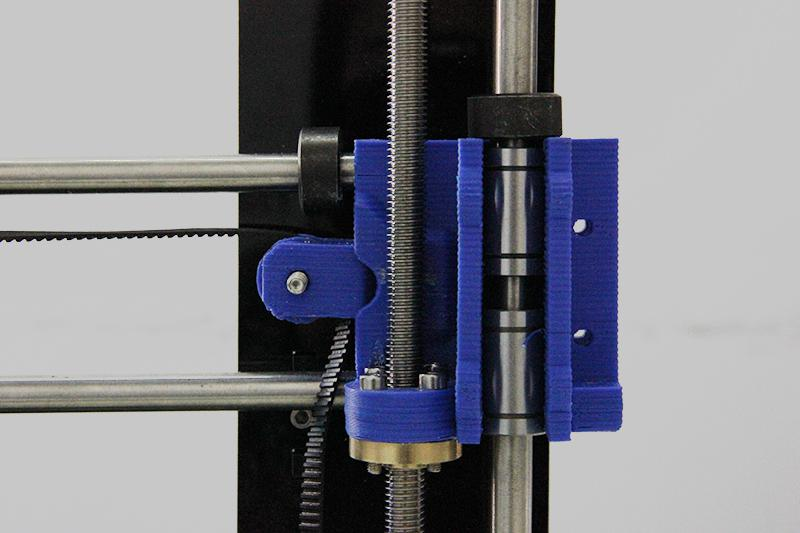
\includegraphics[width=0.3\textwidth]{Bilder/X_Belt_3.jpg} \\ 
\end{tabular}

Die fertige X-Achse kann nun mit den Gewindestangen verschraubt werden. Das Ergebnis sollte nun so (oder ähnlich) aussehen:\\
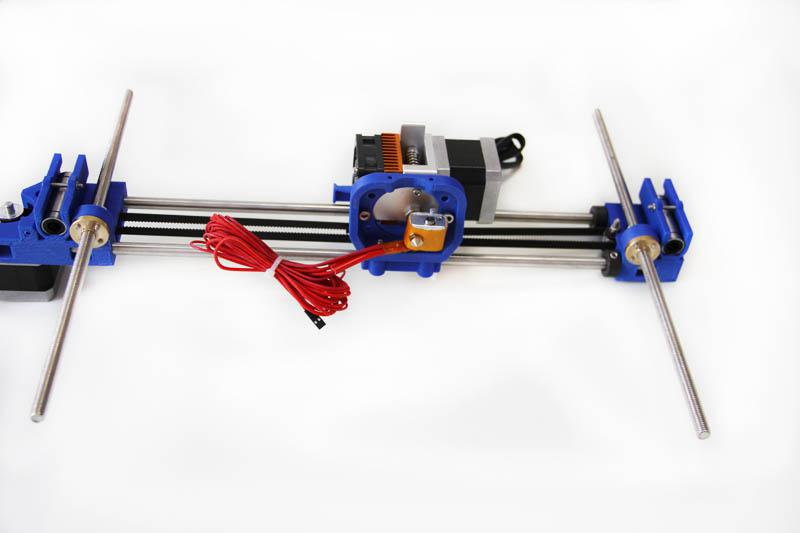
\includegraphics[clip=true, trim=0 100 0 100, width=\textwidth]{Bilder/X_Assembly_3.jpg}

\subsubsection{Aufbau der Z-Achse:}
Nachdem nun die X-Achse fertig gestellt worden ist, kann die Z-Achse endgültig zusammen gebaut werden.
Hierfür müssen zuerst die Z-Motoren mit den Flex-Kupplungen ausgestattet werden, um die Motor-Achsen mit den Gewindestangen zu verbinden:\\
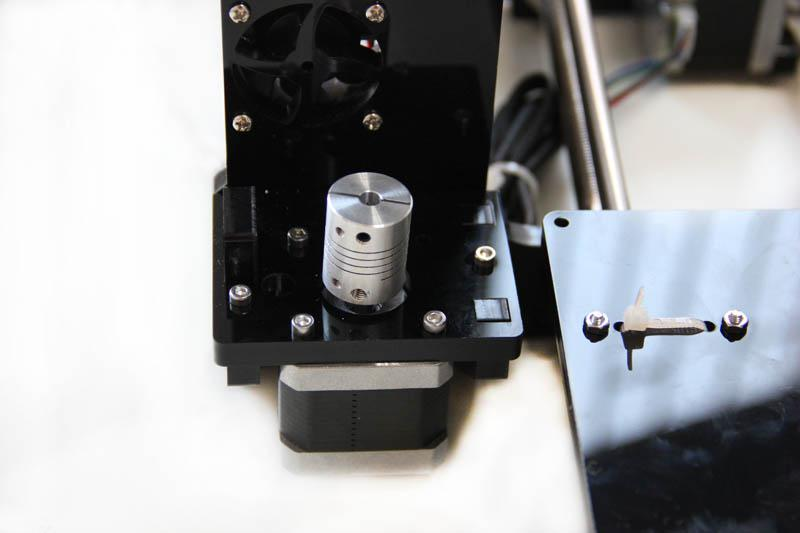
\includegraphics[width=\textwidth, clip=true, trim=0 30 0 70]{Bilder/Z_Assembly_5.jpg}

Danach kann die fertige X-Achse verbunden werden. Hierzu schiebt man zuerst die Gewindestangen der X-Achse in die Kupplungen, und verschraubt diese. Dann können die Linearstangen durch die Linearlager der X-Achse geschoben werden, und unten in die Halterungslöcher eingeführt werden. Hierbei sollte man die oberen Z-Platten bereit halten, um diese nun aufsetzten zu können. Sie halten Gewindestange und Linearstange fest, und sorgen somit für eine angemessene Stabilität der Z-Achse.

Nun sollte das Endergebnis so aus sehen:\\
\begin{tabular}{cc}
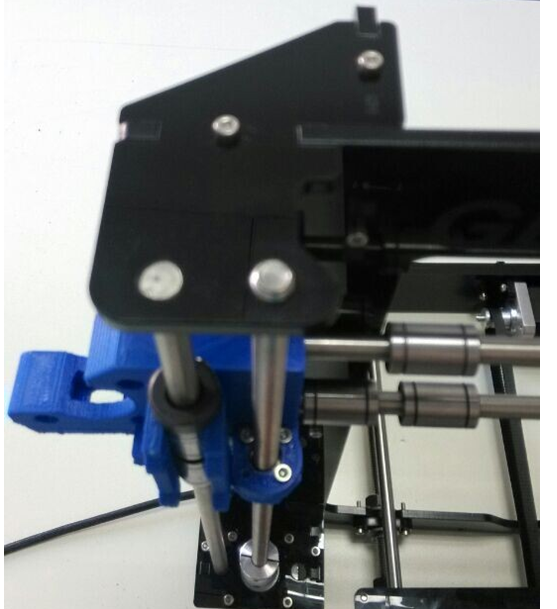
\includegraphics[clip=true, trim= 0 0 30 0, height=0.55\linewidth]{Bilder/Z_Assembly_6.png} & 
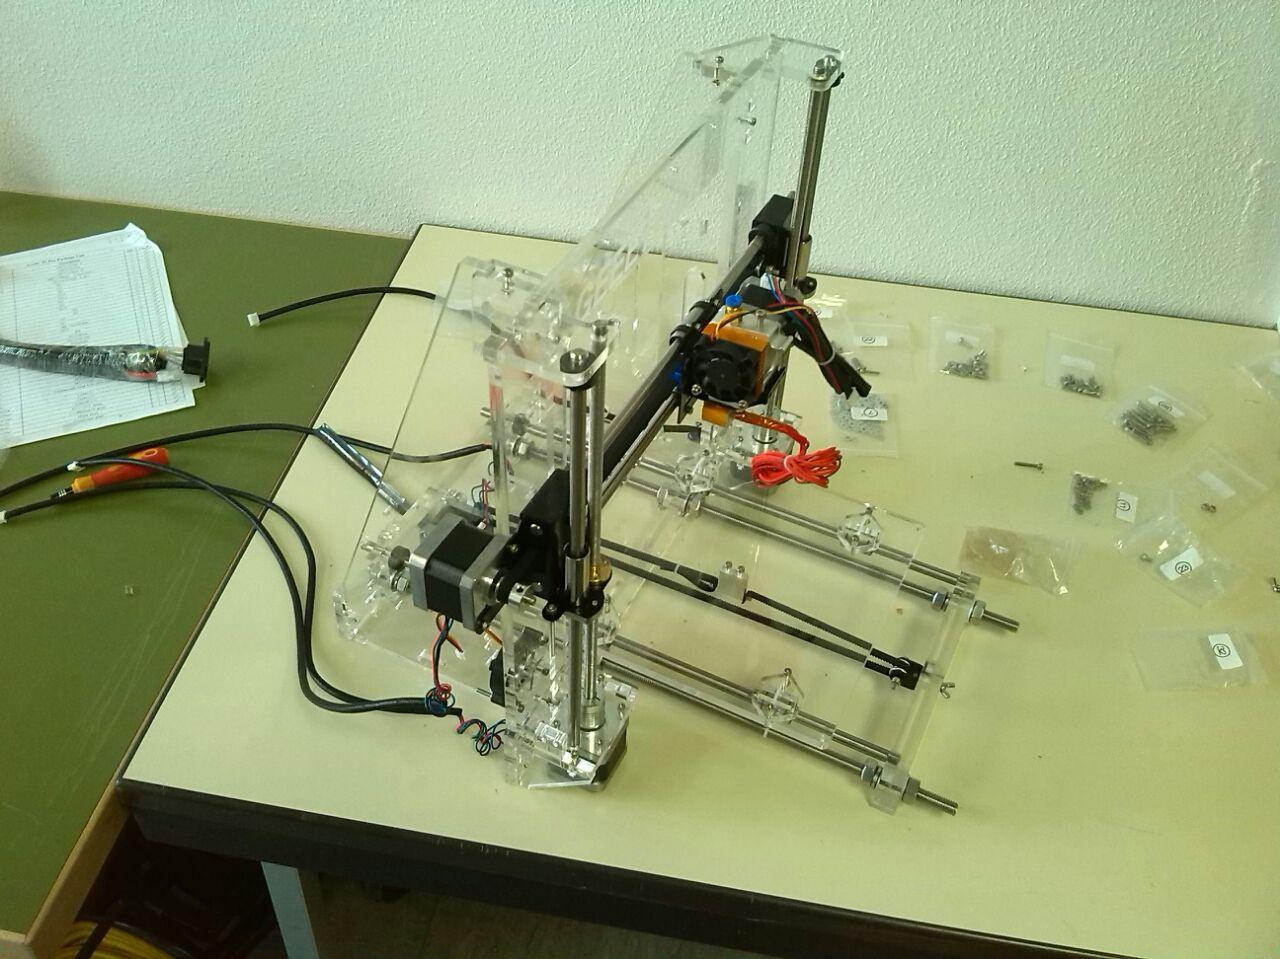
\includegraphics[clip=true, trim= 200 0 150 0, height=0.55\linewidth]{Bilder/XYZ_Merge_1.jpg} \\
\end{tabular}

\subsubsection{Anbringen der Elektronik}
Da nun das gesamte Gestell fertig zusammen gebaut ist, können nun die weiteren Komponenten, so wie z.B. das beheizte Druckbett (Heatbed) oder die Endschalter (Endstops) angebracht werden.

\paragraph{Das Heatbed} kann mithilfe der mit gelieferten M3 Schrauben, sowie den vier Federn, auf dem Y-Achsen-Schlitten angebracht werden. In der Web-Anleitung muss das Heatbed vorher noch verkabelt werden, dies war jedoch für den Schul-Drucker nicht nötig. Ist das Heizbett nun fertig angebracht, so kann die beiliegende Glasplatte mithilfe der Klemmen auf dem Heatbed befestigt werden. Das Endergebnis sollte folgendermaßen aus sehen:\\
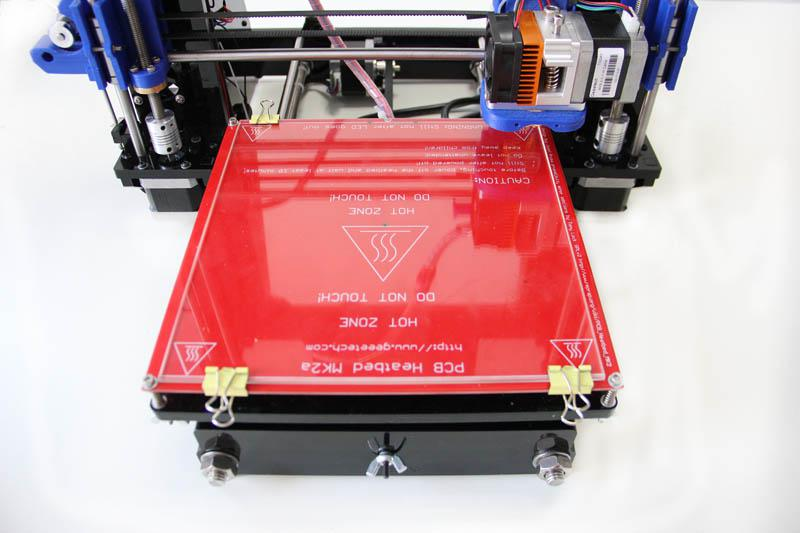
\includegraphics[width=\textwidth]{Bilder/Assembled_BED.jpg}


\paragraph{Endstops:} Nachdem das Bett sicher angebracht ist, können nun die Endstops an der X- Y- und Z-Achse angebracht werden. Sie dienen dazu, dem Drucker seine Position zu identifizieren, und sind damit essentiell für die zuverlässige Funktionalität dessen. Die drei Endstops können wie folgt angebracht werden:\\
\begin{tabular}{ccc}
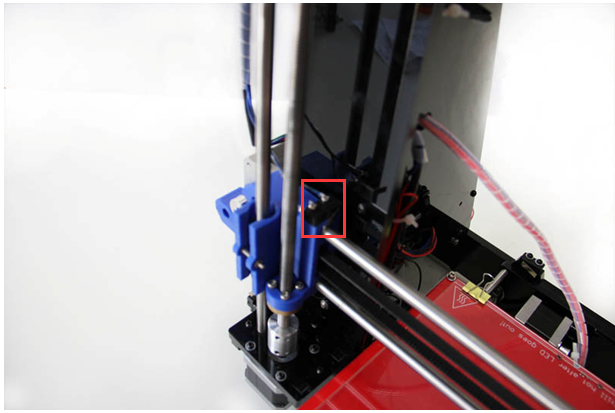
\includegraphics[clip=true, trim=150 80 150 80, width=0.3\textwidth]{Bilder/Endstop_X.png} & 
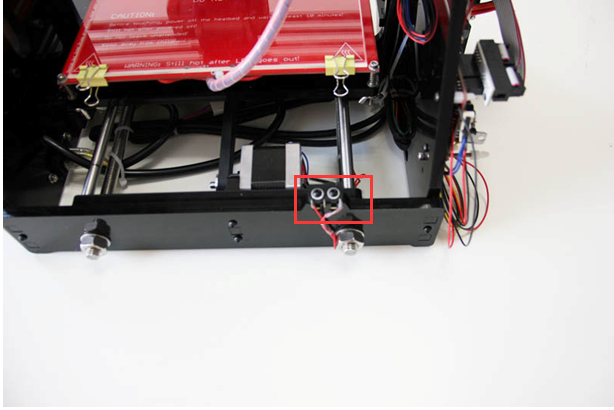
\includegraphics[clip=true, trim=165 80 135 78, width=0.3\textwidth]{Bilder/Endstop_Y.png} & 
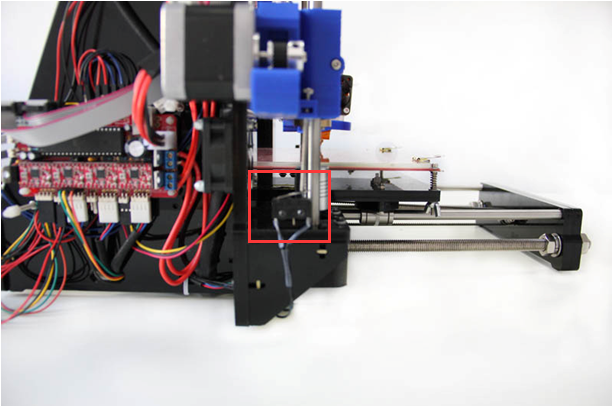
\includegraphics[clip=true, trim=120 60 140 58, width=0.3\textwidth]{Bilder/Endstop_Z.png} \\ 
\end{tabular} 

\paragraph{Das LC-Display} kann nun mit den übrig gebliebenen Teilen fixiert werden. Ob man es hierbei am Frame des Druckers an bringt, oder eventuell eine Halterung dafür druckt und es vor/neben den Drucker stellt ist dem Nutzer überlassen. Am Schuldrucker wurde das LC-Display am Frame folgendermaßen angebracht:\\
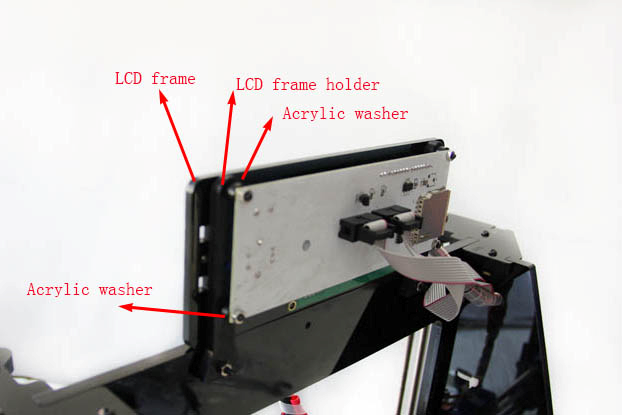
\includegraphics[width=\textwidth]{Bilder/LCD.png}

\paragraph{Die PSU} kann an der (von Vorne) rechten Seite des Frames angebracht werden. Hierfür werden nur einige Schrauben benötigt. Vor dem Einbau sollte darauf geachtet werden, dass die Spannungseinstellung der PSU auf 220V (bzw. 110V falls nötig) eingestellt ist. Falsche Einstellung wird zu Schaden führen! Auch bei der Verkabelung selbst sollte Wert darauf gelegt werden, die einzelnen Kabel korrekt an zu schließen, da ansonsten das Gerät nicht ordnungsgemäß funktionieren wird! 

Die Kabel sollten dabei so aussehen:\\
\begin{tabular}{cc}
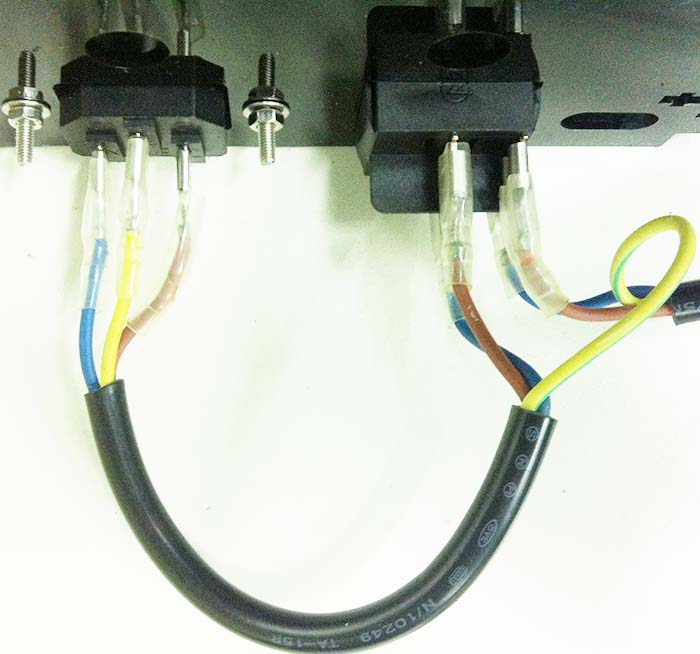
\includegraphics[width=0.5\textwidth]{Bilder/Power_1.jpg} &
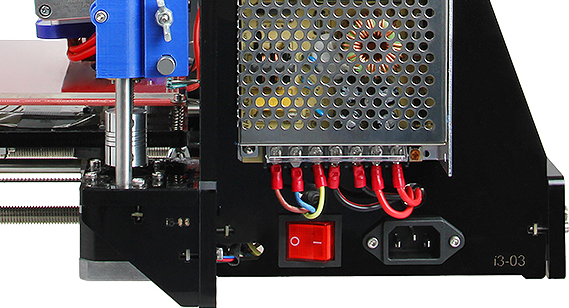
\includegraphics[clip=true, trim=140 0 100 0, width=0.5\textwidth]{Bilder/Power_2.jpg} \\
\end{tabular}

\paragraph{Die Elektronik} kann nun als letztes angebracht werden. Hierfür werden einige Schrauben benötigt, mit denen der PCB an der linken Seite (gegenüber der PSU) angebracht werden kann.\\
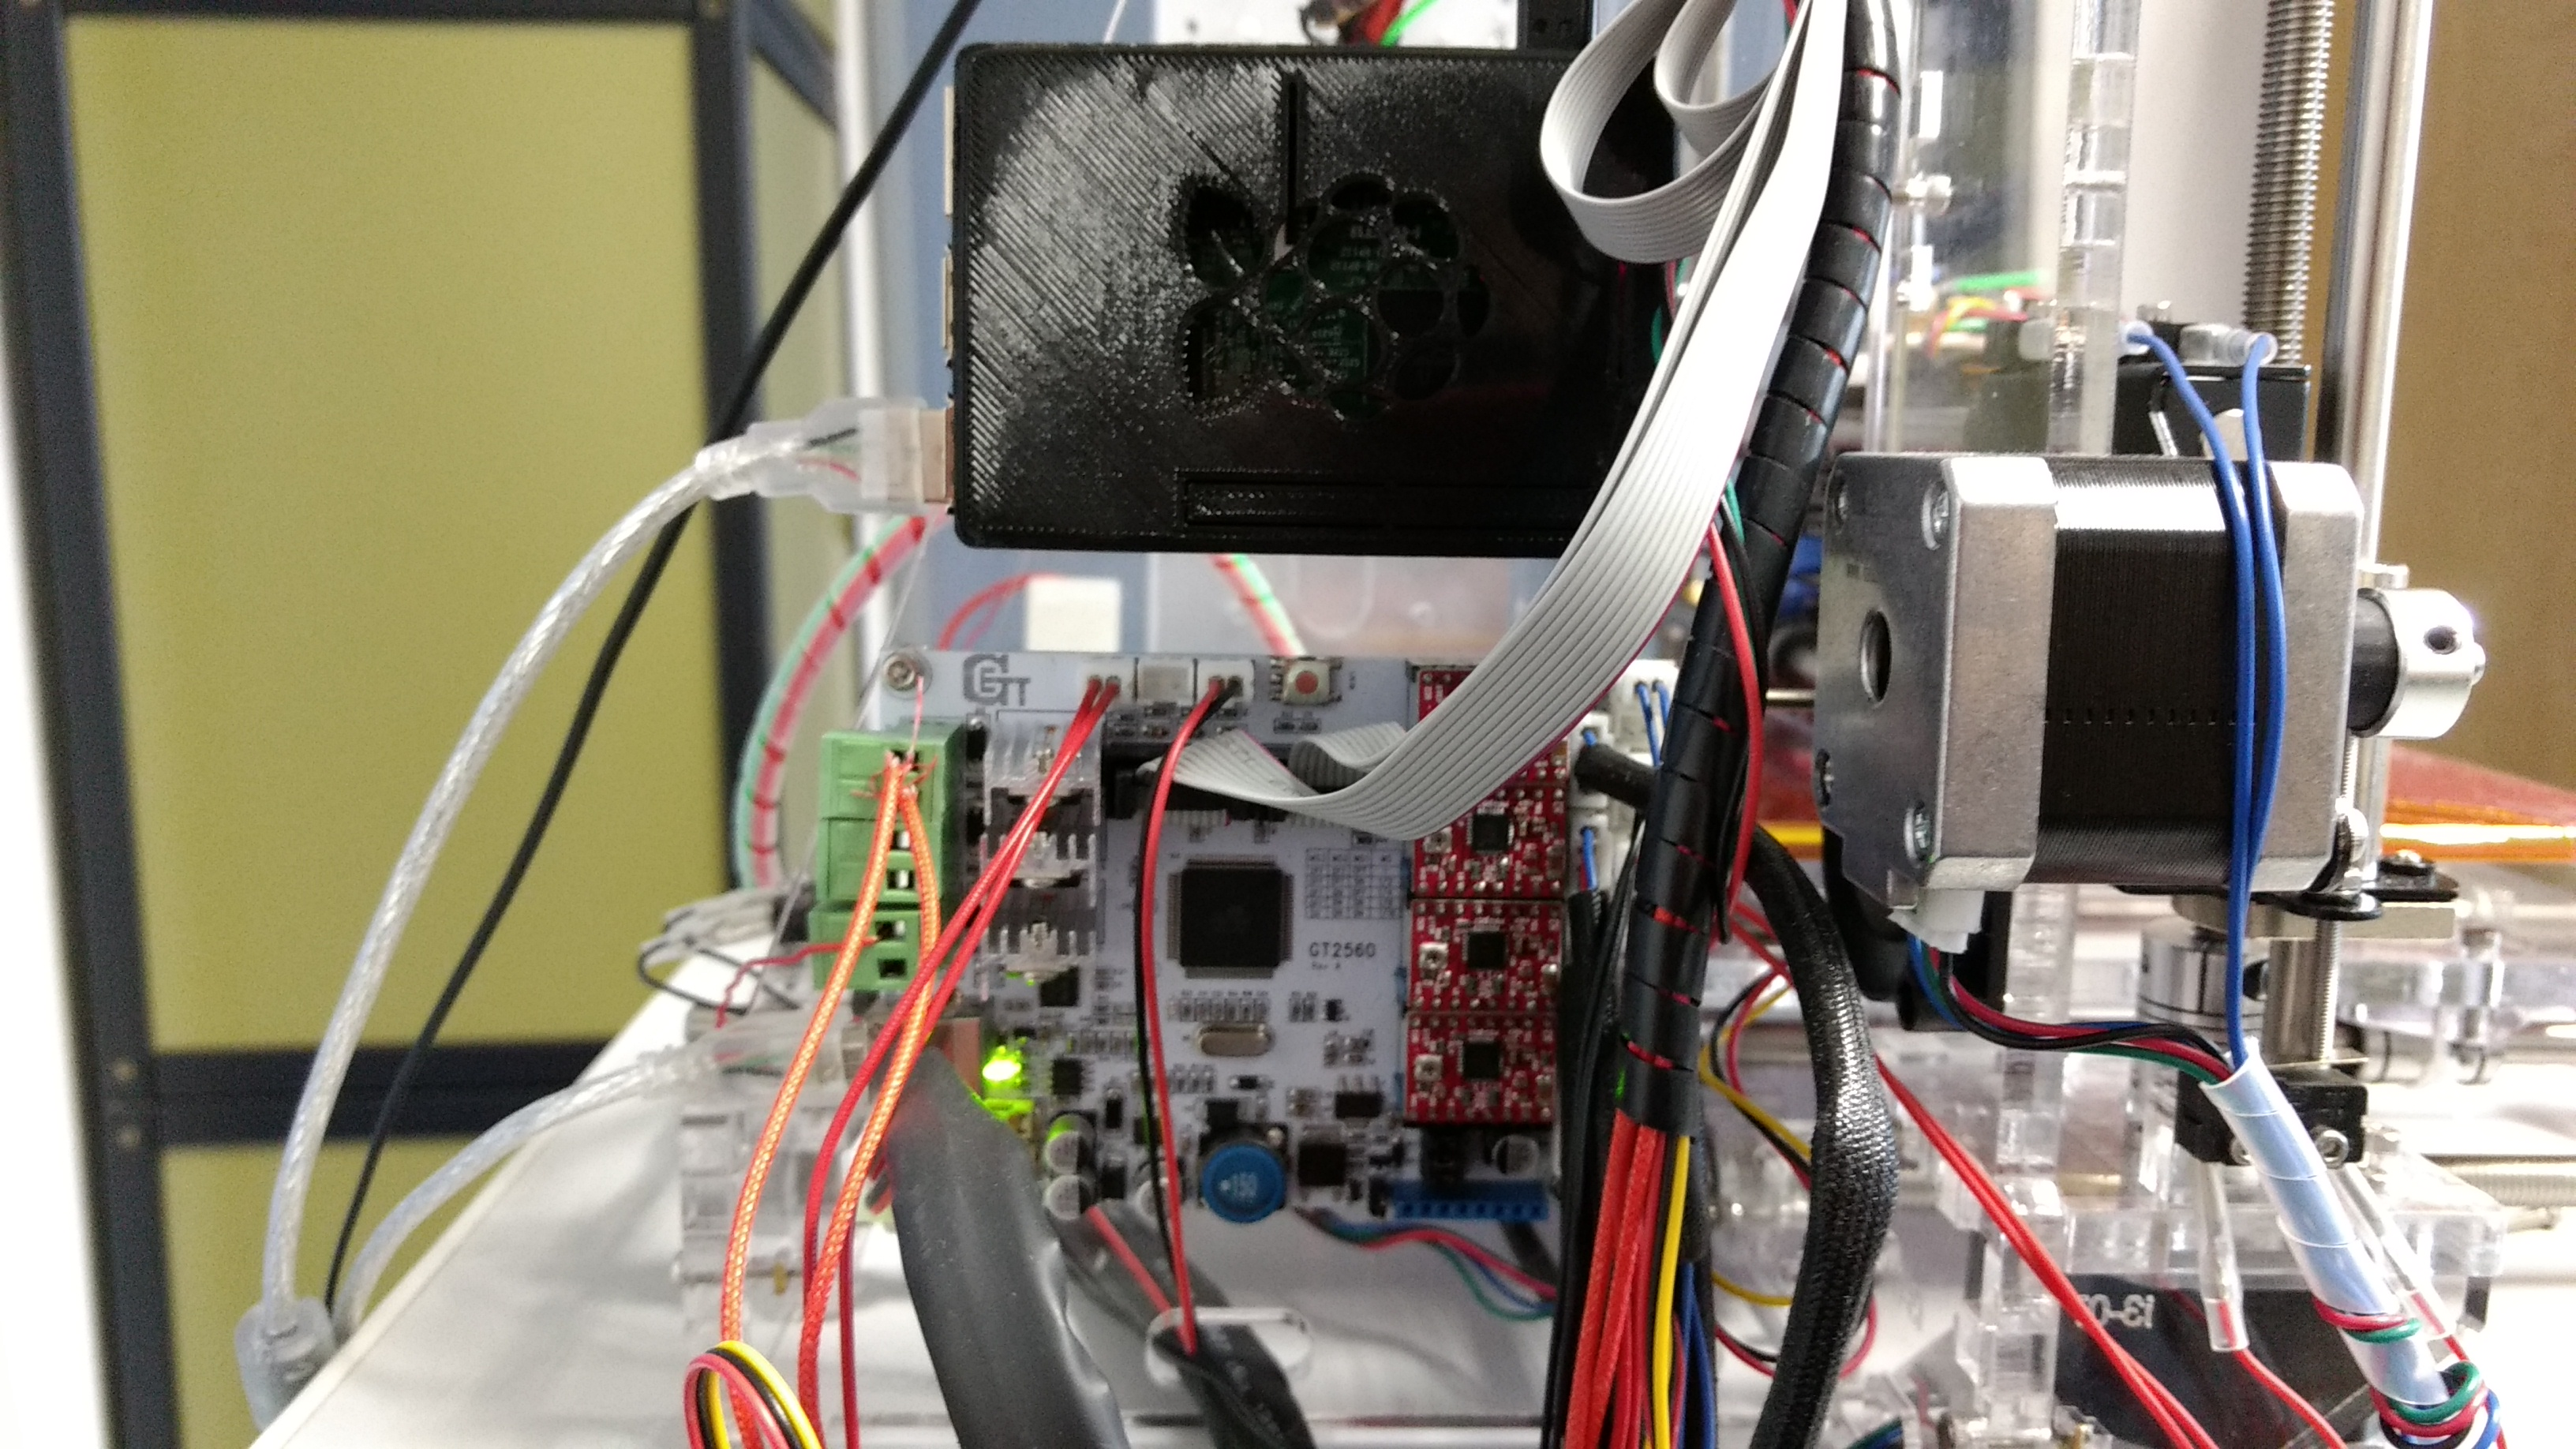
\includegraphics[width=\textwidth]{Bilder/Tutorial/IMG_20161101_143146715.jpg}\\

Nun können die einzelnen Elemente wie Heatbed, Extruder, Motoren und Sensoren am Board angeschlossen werden. Hierbei sollte man eine Board-Spezifische Anleitung befolgen. Für das GT2560, welches in diesem Drucker verwendet wird, sah dies so aus:\\
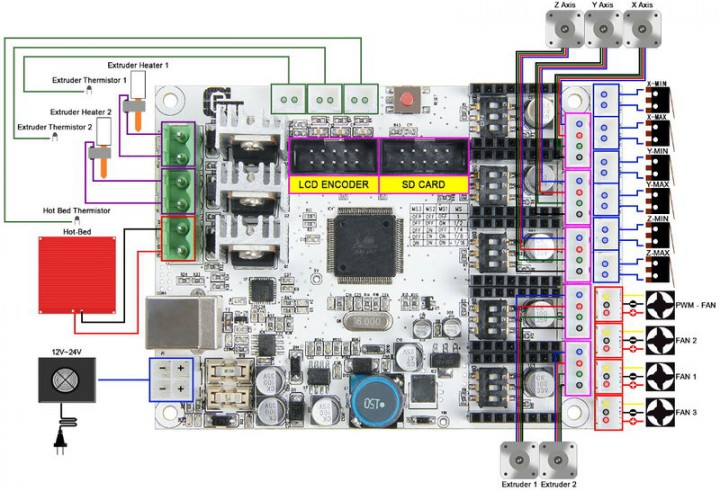
\includegraphics[width=\textwidth]{Bilder/Electronics_2.jpg}

\newpage
\subsubsection{Fertigstellung}
Nachdem alle Kabel verlegt, alle Schrauben gefestigt wurden, und der Drucker auf Funktionalität überprüft ist (durch anstellen und Bewegen einiger Motoren etc.), sollte das Endergebnis folgendermaßen aus sehen:\\
\begin{center}
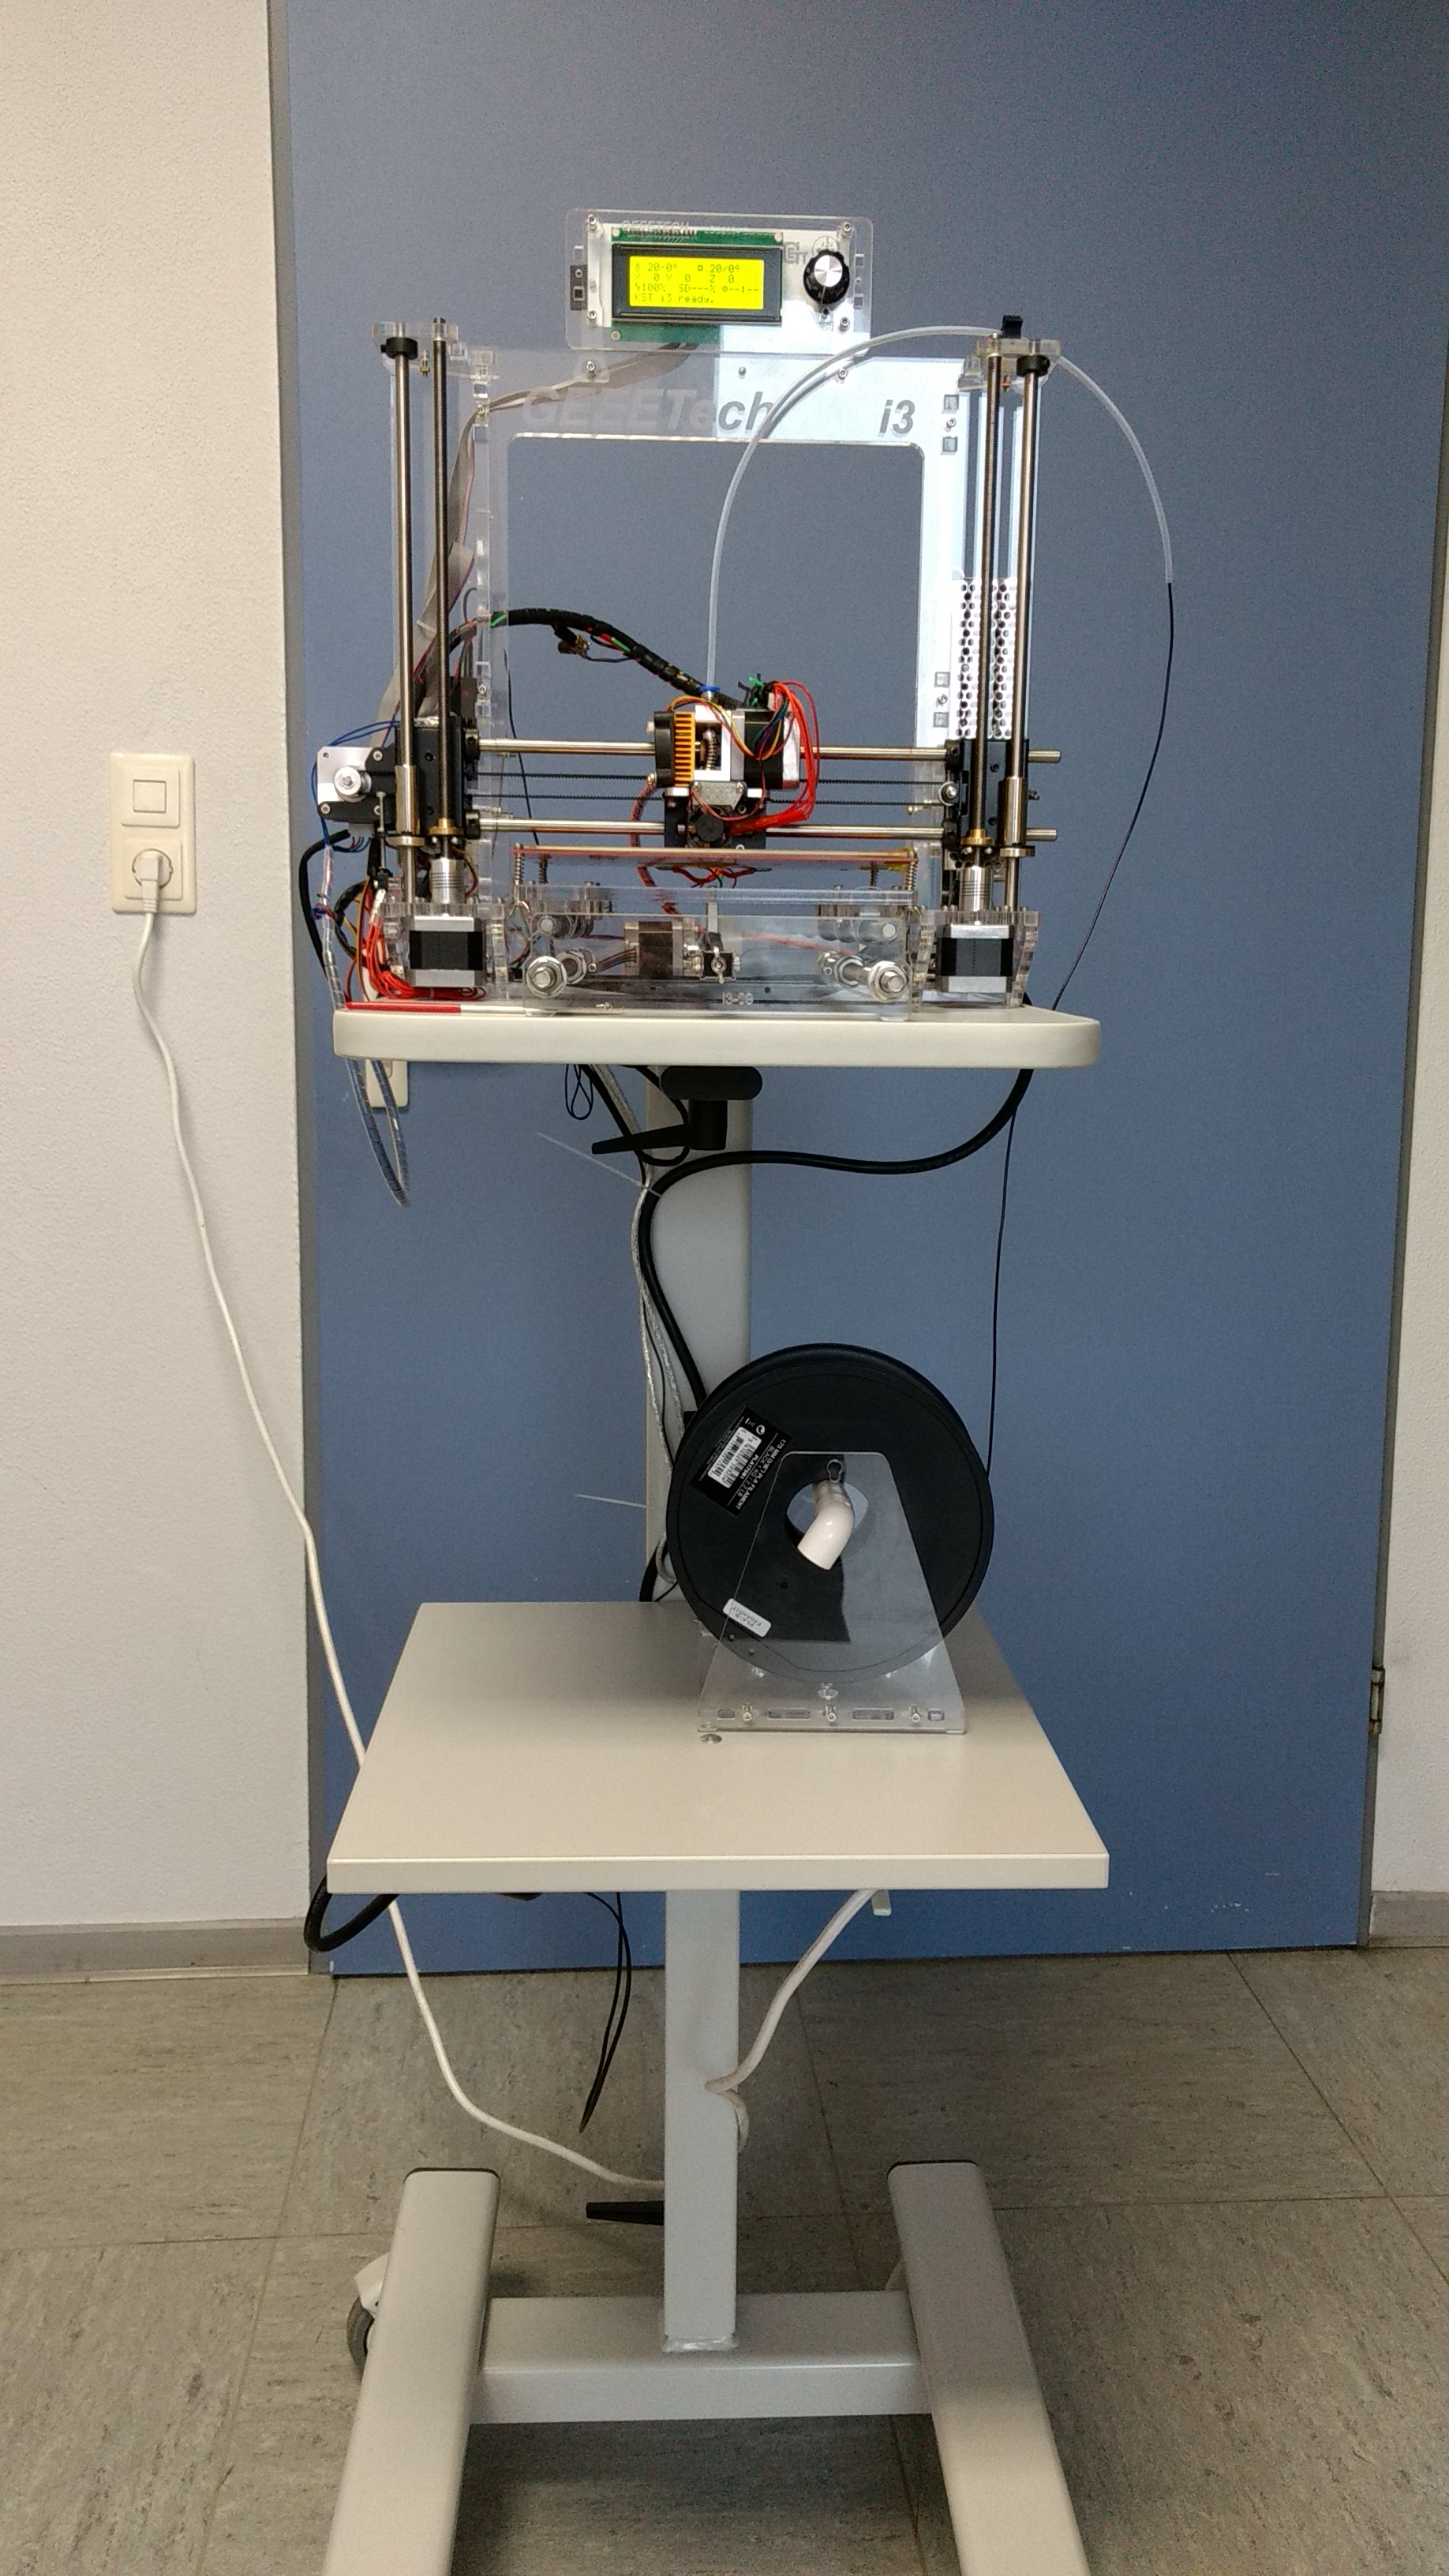
\includegraphics[width=0.7\textwidth]{Bilder/Tutorial/IMG_20161101_143059461.jpg}
\end{center}